\subsection{Introduction to gas fees}
Ethereum\cite{EthereumWhitepaper}  supports  smart  contracts,  meaning  that  some  nodes (validators) of the network have to run the solidity code of these contracts when one wants them. Since  solidity  is  a  Turing  complete  language,  it  remains impossible to say if a given piece of code will terminate and how much resources it will use, it refers to the halting problem which is NP-hard. To avoid malicious people or errors to crash the  network  with  an  infinite  loop,  the  users  of  the  contract provide  a  certain  amount  of  gas $x$ for  each  execution.  When validators  execute  smart  contracts  they  decompose  the  code into basic low-level operations. Each of these operations ($o$) is also associated with a fixed amount of Gas ($Gas(o)$). Then, for each executed operation ($o$) the validator subtract (pay himself) $Gas(o)$ from $x$.  If  $x$  goes  to  $0$  the  execution  terminates,  in this  case,  the  operations  of  the  contract  are  reverted  but  the Gas is not refunded to the user. Since gas has a real price (in ETH/Gwei), it is impossible (with a finite amount of money) to create an infinite loop. The amount of gas used by an operation is determined by the low-level instructions. However, the price paid for each gas is driven by offer and demand. The validator shave  the  choice  to  validate  any  operation  from  a  pool.  Each user  can  associate the  gas  price  he  wants with  his  operation. Since  the  validators  get  paid  with  the  gas  their  incentive  is to validate operations with the highest gas prices. This is the reason why the gas price can spike when the network is busy, users are willing to pay more to get their operations validated faster.
\subsection{Gas prices and volume}
Gas prices are driven by supply and demand for the network's processing capacity, which is required to perform smart contracts and other transactions.
When the Ethereum network is experiencing a large volume of transactions, gas can become expensive. Moreover, the number of transactions that can be included in each new block uploaded to the Ethereum blockchain is limited. Therefore, miners are incentivised to accept transactions at greater gas fees due to supply and demand. As of November 2021, the daily amount of Gas used Per Day is roughly 100 billions, and it increases every day, see Figure \ref{fig:gas_volume}. 

\begin{figure}[htbp]
    \caption{Chart representing 5 years of historical data on Gas volume.}
    \label{fig:gas_volume}
\end{figure}

Another problem related to gas is its volatility. On Figure \ref{fig:gas_prices}, we can see one year of historical data on Gas prices, providing evidence for large variation in prices. In fact, looking further in time, we observe that certain events can even make Gas prices skyrocket (see Figure \ref{fig:gas_prices5}. This, together with the incredibly high and still increasing Gas volume, deter possible investors from using DeFI (Decentralized Finance) protocols. 

\begin{figure}[htbp]
    \centerline{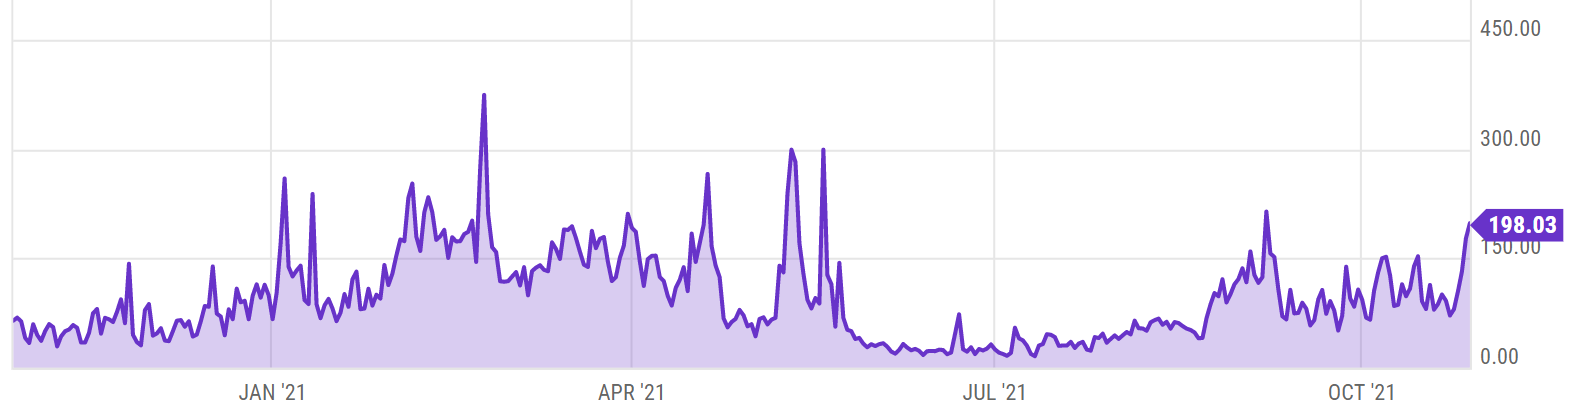
\includegraphics[width=90mm]{figures/gas_prices.PNG}}
    \caption{Chart representing 1 year of historical data on Gas prices.}
    \label{fig:gas_prices}
\end{figure}

\begin{figure}[htbp]
    \centerline{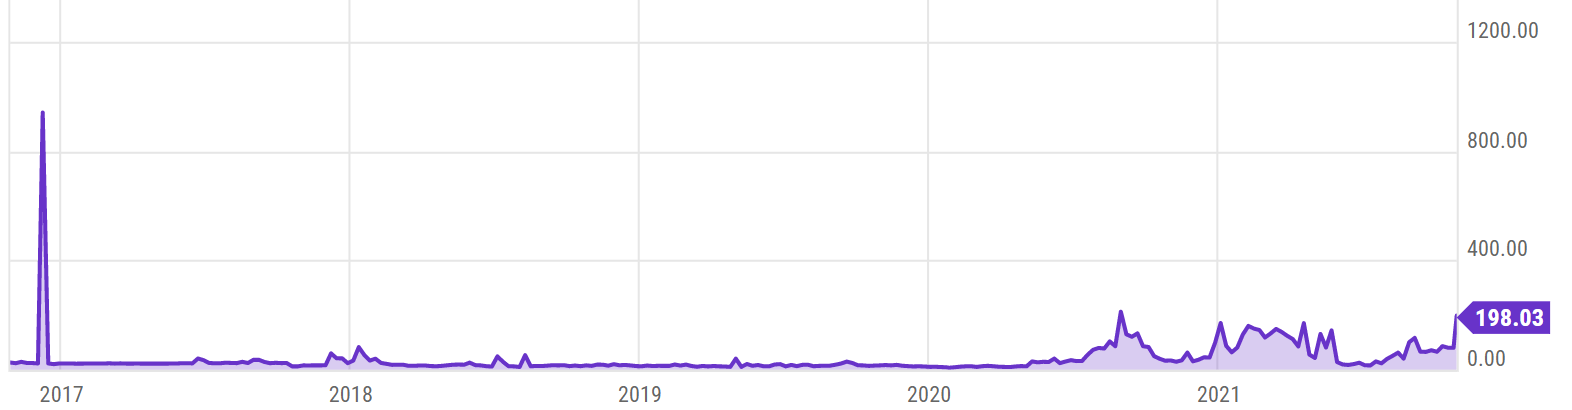
\includegraphics[width=90mm]{figures/gas_prices5.PNG}}
    \caption{Chart representing 5 years of historical data on Gas prices.}
    \label{fig:gas_prices5}
\end{figure}


\subsection{Projects built on Ethereum}
In the previous section, we stated that one of the problems related to Gas is the high volume of Gas used per day. The main reason why these numbers are so high is that there are lots of projects built on the Ethereum blockchain, which we will refer to as Layer 1. Currently, it amounts to 220 DeFi projects. It is important to notice that the Gas consumption is not uniformly distributed among all the projects. For instance, \textit{Uniswap}\cite{adamsUniswapV2Core} is one of the projects that consumes the most, with an average consumption of a 6\% of all the Layer 1 Gas. As a matter of fact, \textit{Uniswap} is only surpassed by \textit{OpenSea}\cite{OpenSeaDeveloperDocumentation}, with a 14\%. 

All in all, Gas fees are becoming an increasing problem that could prevent users from using the Ethereum network. However, these problems also make engineers think about possible solutions, such as the ones that we'll propose on this article.